

\documentclass[11pt]{article}

\title{ Advancing predictive physical modeling through focused development of model systems to drive new modeling innovations}

\usepackage[top=0.5in, bottom=0.5in, left=0.5in, right=0.5in]{geometry}
\usepackage{helvet}
\usepackage{url} % hypderref?
\usepackage{graphicx}
\graphicspath{{figures/}} % The figures are in a figures/ subdirectory.
\renewcommand{\familydefault}{\sfdefault}
\pagestyle{empty}
%\pagestyle{plain}

% Fancy page-width tables
\usepackage{tabularx}

% Use a package for framed boxes
\usepackage{mdframed}

\usepackage[T1]{fontenc}
\usepackage{amssymb}


\usepackage{setspace}
\usepackage{microtype}

\usepackage{amsfonts}
\usepackage{amsmath}

\usepackage{floatrow}

\usepackage[normalem]{ulem} % for nci.bst

\usepackage{sidecap}
\usepackage[abs]{overpic}
\usepackage{wrapfig}


\usepackage{hyperref}
\hypersetup{colorlinks=true, urlcolor=black, citecolor=black, linkcolor=black}

\usepackage[numbers,sort&compress]{natbib} %comment on first run?

\usepackage{multibib}
%\newcites{full,sampl}{A,B}
\newcites{sampl}{Full List of SAMPL References}
%\newbibliography{full}

%\usepackage[round,authoryear]{natbib}
%\usepackage{cite}
%\setlength{\bibsep}{0.00in}


\newcommand{\doi}[1]{\href{http://dx.doi.org/#1}{doi:#1}}

\newcommand{\ac}[1]{{\sc \lowercase{#1}}}

\renewcommand{\baselinestretch}{.93}
%\renewcommand{\baselinestretch}{.90}
\usepackage{wrapfig}

\usepackage{bibspacing}
\setlength{\bibspacing}{\baselineskip}




\graphicspath{{figs/}}

\makeatletter

\newcommand{\captionfonts}{\footnotesize}

\makeatletter  % Allow the use of @ in command names
\long\def\@makecaption#1#2{%
  \vskip\abovecaptionskip
  \sbox\@tempboxa{{\captionfonts #1: #2}}%
  \ifdim \wd\@tempboxa >\hsize
    {\captionfonts #1. #2\par}
  \else
    \hbox to\hsize{\hfil\box\@tempboxa\hfil}%
  \fi
  \vskip\belowcaptionskip}
\makeatother

\renewcommand{\figurename}{{\bf Figure}}

% Page numbering.
%\pagestyle{plain}
%\pagenumbering{arabic}

\setlength{\abovecaptionskip}{-5pt}

\makeatother

\renewcommand{\refname}{Bibliography and References Cited}

\setlength{\parindent}{0pt} % Don't indent first line
%\setlength{\parskip}{1ex plus 0.5ex minus 0.2ex} % Add some space between paragraphs
\setlength{\parskip}{0.8ex} % Add some space between paragraphs

\begin{document}

\textbf{Doctoral Dissertation and Prior Research Experience}\\
Over the course of my graduate work I have developed the first example of multicomponent bioluminescence imaging with synthetic probes and gained broad experience in the areas of chemical biology and reaction methodology. These efforts combined my skills in chemical synthesis, biological assay development, and computer programming. My work has wide implications in the fields of imaging and protein engineering.

%%%%%%%%%%%%%%%%%%%%%%%%%%%%%%%%%%%%%%%%%%%%%%%%%%%%%%%%%%%%%%%%%%%%%%%%%%%%%%%%
%Chemiluminescence
\begin{wrapfigure}[6]{r}{8cm}
\vspace{-0.2in}
\begin{centering}
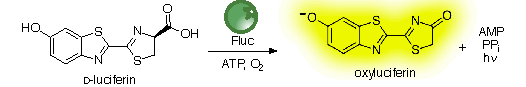
\includegraphics[width=\textwidth]{figures/Previous_research/luc_oxidation.pdf}

\end{centering}
\footnotesize
\caption{\label{figure:chemilum}
Oxidation of D-luciferin by firefly luciferase (Fluc) produces a photon of light.
}
\end{wrapfigure}
%%%%%%%%%%%%%%%%%%%%%%%%%%%%%%%%%%%%%%%%%%%%%%%%%%%%%%%%%%%%%%%%%%%%%%%%%%%%%%%%

\textbf{Expanding the imaging toolkit}\\
Genetically-encoded optical reporters have revolutionized our understanding of biological systems. These tools, namely fluorescent proteins, allow researchers to track multiple targets over extended periods of time in cellulo. However, the transition of fluorescent probes in vivo, to multicellular clinical models, has been hampered by the opacity of tissue and its propensity for autofluorescence. A complementary imaging technology, bioluminescence, does not suffer from these complications because it does not require excitation light.
% TODO ref a review? Rice?
Thus, the technique is exquisitely sensitive—with the ability to see as few as ten cells—and is often more suitable for imaging in thick tissues and entire organisms. Bioluminescence relies on luciferase enzymes that catalyze the oxidation of small-molecule substrates (luciferins), releasing photons of light in the process (Fig. \ref{figure:chemilum}). Unfortunately, the optimal luciferases for in vivo use rely on the same small molecule luciferin, precluding studies of more than one feature or cell type at a time.

To address this issue, I developed and analyzed a number of new luciferin probes, and created a selection platform to find mutually orthogonal luciferases and luciferins for multicomponent imaging. In contrast to the spectroscopic resolution of fluorescent tools, these probes were designed to exhibit substrate resolution. Since red light is the only color capable of penetrating tissue, spectral resolution in vivo is difficult to achieve.
% TODO Rice Contag JBiomedOpt 2005??
Thus, I resolved to take advantage of the molecular component of bioluminescence imaging to develop exclusively selective luciferin-luciferase pairs.

\textit{Brominated luciferins are versatile bioluminescent probes}\\ % QUESTION get rid of all of this??
My strategy for mutually selective probes relied on synthesizing small molecule luciferin analogs and screening them against libraries of functional mutant luciferases. I initially focused on development of minimally perturbed luciferin probes. We rationalized that bromination of the luciferin core might perturb binding to the wildtype enzyme, yet retain inherent light-emitting ability of the molecule. Directed evolution could then be used to restore light emission. To verify this, I developed a chemiluminescence assay to test the relative light-emitting abilities of our luciferin analogs (Figure 1B). Gratifyingly, the brominated probes showed robust emission, indicating that these molecules had the potential to be capable emitters (Figure 1C). Additionally, I have shown that cross-coupling reactions can be used to derivatize the brominated luciferins, producing a variety of modified scaffolds in a divergent manner. This work resulted in a publication in ChemBioChem.4 In addition to the brominated variants, my colleagues and I synthesized a wide variety of modified luciferins analogs—ranging from subtle electronic modifications, to large steric perturbations. The chemiluminescence assay has proven general for these analogs as well, providing a benchmark for light emission before mutant luciferases are developed.

%%%%%%%%%%%%%%%%%%%%%%%%%%%%%%%%%%%%%%%%%%%%%%%%%%%%%%%%%%%%%%%%%%%%%%%%%%%%%%%%
%Parallel Screening TODO maybe add a hit back in to the fig as (B)
\begin{wrapfigure}[12]{l}{8cm}
\vspace{-0.2in}
\begin{centering}
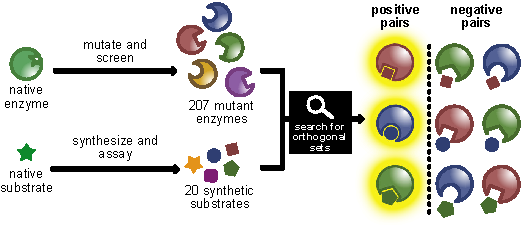
\includegraphics[width=\textwidth]{figures/Previous_research/algorithm_v4.pdf}

\end{centering}
\footnotesize
\caption{\label{figure:algorithm}
Strategy for developing orthogonal bioluminescent probes.
}
\end{wrapfigure}
%%%%%%%%%%%%%%%%%%%%%%%%%%%%%%%%%%%%%%%%%%%%%%%%%%%%%%%%%%%%%%%%%%%%%%%%%%%%%%%%

\textit{Orthogonal Luciferase-luciferin pairs for bioluminescence imaging}\\
Next, we sought to identify luciferase mutants that selectively utilized our luciferin analogs. We designed and generated a range of functional luciferases that reflected a variety of mutations about the active site. Combining molecules and enzymes, we tested 20 luciferins with 207 mutant luciferases (Fig. \ref{figure:algorithm}). The screening experiment generated 4,140 enzyme-substrate combinations, and thus a potential for more than 4 million possible sets of two substrates and two enzymes. Since it would be impractical to evaluate all of these combinations manually, I first derived a mathematical quantification of orthogonality to ‘score’ each potential pairing. Next, I wrote a supercomputer algorithm to search this dataset in a matter of minutes for the highest-scoring pairs. The software provided a ranked list of mutually orthogonal enzyme-substrate pairs that were biochemically verified. A top hit from this list is shown in Figure 2C. Each enzyme exhibited greater than ten-fold preference for its matched substrate. Resolution was maintained when these probes were moved into mouse models, highlighting the speed and accuracy of our approach (Figure 3A). As a next step, I have been searching the data sets for not just pairs of bioluminescent tools, but triplet and quadruplet sets of orthogonal probes. This would enable visualization of three or more populations of interest simultaneously. However, the problem becomes much more complex due to the increase in possible pairings (Figure 2A). Using my algorithm, I have identified 6,171 possible sets of orthogonal triplets, several of which have been verified in bacterial lysate (Figure 3B). This work resulted in a publication in JACS,5 with an additional manuscript submitted to ACS Central Science.6 We hope to use these tools to monitor the locations of cancer cells and the immune system throughout disease progression. Collectively, our orthogonal pairs will enable a variety of multicomponent, in vivo imaging studies, and my screening techniques and computer algorithm will enable advances in other areas of chemical biology.

%%%%%%%%%%%%%%%%%%%%%%%%%%%%%%%%%%%%%%%%%%%%%%%%%%%%%%%%%%%%%%%%%%%%%%%%%%%%%%%%
%In vivo imaging TODO update this fig??
\begin{wrapfigure}[20]{r}{7cm}
\vspace{-0.2in}
\begin{centering}
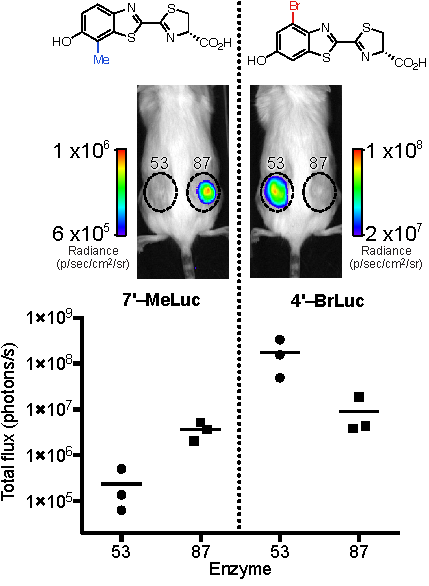
\includegraphics[width=\textwidth]{figures/Previous_research/just_mice.pdf}

\end{centering}
\footnotesize
\caption{\label{figure:mice}
Mutually orthogonal pairs enable multicomponent imaging in mouse models.
}
\end{wrapfigure}
%%%%%%%%%%%%%%%%%%%%%%%%%%%%%%%%%%%%%%%%%%%%%%%%%%%%%%%%%%%%%%%%%%%%%%%%%%%%%%%%

\textit{Expanding the scope of multicomponent imaging}\\
My most recent work has focused on increasing the practicality of these tools for preclinical in vivo imaging. The major drawbacks of our substrate resolution approach include temporal resolution and background emission. I am addressing these issues by utilizing traditional spectral unmixing algorithms to deconvolute substrate signals mathematically. This will enable sequential imaging of substrates, and the ability to resolve smaller numbers of cells. We are currently testing this technique in mouse models. Additionally, I am evaluating new libraries of luciferases via deep sequencing to elucidate selectivity trends in modified luciferins. % TODO more here!!

%%%%%%%%%%%%%%%%%%%%%%%%%%%%%%%%%%%%%%%%%%%%%%%%%%%%%%%%%%%%%%%%%%%%%%%%%%%%%%%%
% TODO some multicomponent fig Here
%%%%%%%%%%%%%%%%%%%%%%%%%%%%%%%%%%%%%%%%%%%%%%%%%%%%%%%%%%%%%%%%%%%%%%%%%%%%%%%%

\textbf{Previous work in transition metal catalysis methodology}\\
I spent the first year and a half of my graduate work in the lab of Professor Vy Dong. During this time, I sought new, streamlined methods of carbohydrate synthesis. We developed a new method of selectively acylating sugars via copper catalysis.7 Our catalysts could distinguish between three similar alcohols moieties to acylate at a set position, depending on the ligand used. This method proved general for a variety of sugar scaffolds containing cis diols.


\eject

%\footnotesize
%\scriptsize
%\bibliographystyle{acm}
%%\bibliographystylesampl{nci}
%%\bibliographystyle{nci}
%\bibliographystyle{nar}
%\bibliography{full}{sampl-r01}{BIBLIOGRAPHY AND REFERENCES CITED}
%\bibliography{sampl}{sampl-r01}{REFERENCES FROM PRIOR SAMPL CHALLENGES}

%%\bibliographysampl{sampl}
\eject
%%\bibliography{sampl-r01}

\end{document}
